\chapter{Introduction — phonology}
\label{cha:introduction-phonology}
In Modern Welsh, voiceless stops — \mw{p, t, c} — are now lenited to \mw{b, d, g}.  This thesis argues that these lenited voiceless  stops (\lT)  did not initially merge with unlenited voiced stops — \mw{b, d, g} (\xD). More specifically, it argues that the phonological variables keeping these phonemes are recoverable, and that \lT\ and \xD\ were still separate phonemes well into the \gls{mw} period. The thesis is divided in two parts, and Part~\ref{part:phonology-phonetics}  treats which phonological variables kept these sounds apart in Welsh, while Part~\ref{part:orthography} addresses the date when \lT\ and \xD\ merged. This chapter introduces the concept of lenition and some of the history of scholarship on lenition in Celtic, focusing on the idea that \lT\ did not equal \xD\ word-initially in Brittonic. It then concludes this literature review by introducing my own reconstruction of how \xT, \lT, and \xD\ were kept apart in post-\gls{apoc} Brittonic. 

\begin{table}[h]
  \centering
  \begin{tabular}{lllll}
    \toprule
    & \multicolumn{2}{c}{Modern Welsh} & \multicolumn{2}{c}{Old Irish} \\
    & Radical & Lenited & Radical & Lenited \\\midrule
    \gls{T} & /p t k/ & \emph{/b d ɡ/}
    & /(p) t k/ & /(f) θ x/  \\
    \gls{D} & \emph{/b d ɡ/} &  /v ð \zero/
    & /b d ɡ/ & /β ð ɣ/ \\
    \bottomrule
    \multicolumn{5}{p{0.5\textwidth}}{\footnotesize The table is simplified for Old Irish: it does not distinguish palatal and non-palatal phonemes.}
  \end{tabular}%
  \caption{Radical and lenited stop consonants in Modern Welsh and Old Irish.}
  \label{tab:lenitionwelshirish}%
\end{table}%

Lenition is a morphophonemic process found in all Celtic languages. This means that the first consonant of a word may change into a more sonorous one as a result of its morphosyntactic environment; however, the way in which a consonant is made into a more sonorous one differs between the Goidelic and the Brittonic branches of Celtic\footnote{The Goidelic languages comprise Old Irish and its descendants Irish, Scottish and Manx Gaelic. The Brittonic languages comprise Welsh, Cornish and Breton.}. In Goidelic, all stop consonants turn into their fricative counterparts, while present-day Brittonic voiceless stops turn into their voiced counterparts and voiced stops turn into their respective fricatives. Table~\ref{tab:lenitionwelshirish} shows the differing treatments between Brittonic and Goidelic using Modern Welsh and Old Irish as examples. Here, the emphasised areas indicate a merger in Welsh not found in Irish. Judging from their Old Irish counterparts alone we can see that lenited voiceless stops  and radical voiced stops  must at some point have been separate in Brittonic as well.

\section{A two-stage development of lenition}
\label{sec:two-stage-devel}
Goidelic and Brittonic both have the morphological instrument of lenition, but the phonemes used to express lenition differ. How can we account for the emergence of lenition in a single theory in spite of this difference? A unified theory that accounts for both Goidelic and Brittonic would require several steps. Yet early scholars of Welsh  frequently described lenition as just one sound law. An example of a historical grammar of Welsh describing lenition as such is \textcite{Mor_Welsh13}, who notes the following on lenition:
\tqt{Brit.\ and Lat. \textit{p, t, k, b, d, g, m} between vowels became \textit{b, d, g, f, δ, ᵹ, f} respectively in W.}{Mor_Welsh13}{§~103}
This description gives a correct summary of the totality of changes between \gls{pbr} and \gls{mow}, but does not separate these changes  into intermediate stages. 
Yet when he posits that present-day Brittonic languages /p t k/ lenite to /b d ɡ/, he makes two claims: the first is that lenition was applied to voiceless stops at some point in the history of Brittonic; the second is that the phonemes to which these voiceless stops lenited were merged with the pre-existing phonemes /b d ɡ/. These two developments may be taken together by scholars of \eg Welsh, because that is the final result in present-day Welsh; however, failing to separate these two developments  creates a few problems.

One obvious problem is that if the two Brittonic developments occurred in a single step, then lenition in Goidelic and Brittonic cannot be described as a single development, because Goidelic voiceless stops lenite into /f θ x/, and it is hard to derive the Goidelic  voiceless fricatives from the Brittonic voiced stops, or vice versa. Another problem is Brittonic-internal. If voiceless stops after lenition came to equal unlenited voiced stops immediately, then would these not have to be lenited into lenited voiced stops in turn? This issue is recognised  by \textcite{loth_les_1892}, who proposes that voiceless stops underwent lenition at a later date than other consonants:
\tqt{\textfrench{Les explosives sonores \textit{b, d, g}, entre deux voyelles ont dû \textit{commencer} leur mouvement vers les spirantes correspondantes, avant que les explosives sourdes, \textit{p, t, c} ne fussent devenues \textit{b, d, g}; autrement, celles-ci auraient eu le même sort qu'elles. Si le latin \textit{opera} avait donné \textit{obera} au moment où \textit{labore} était encore \textit{labure}, le \textit{b} d'\textit{ober} eût été traité comme celui de \textit{labur}; c'est-à-dire fût devenu \textit{v}; on aurait aujourd'hui \textit{over, lavur} et non \textit{ober, lavur}. Des trois explosives sonores, \textit{g} paraît la première être devenue spirante.}\footnote{The voiced stops \textit{b, d, g} between two vowels must have \emph{started} their movement towards their corresponding spirants before the voiceless stops became \textit{b, d, g}; otherwise, these ones would have had the same fate as those. If Latin \textit{opera} had given \textit{obera} at the moment when \textit{labore} was still \textit{labure}, the \textit{b} of \textit{ober} would have been treated as the one of \textit{labur}; \ie it would have become \textit{v}; today we would have \textit{over, lavur} and not \textit{ober, lavur}. Of the three voiced stops, \textit{g} seems to be the first to have become a spirant.}}{loth_les_1892}{87}
Loth's explanation accounts for why a consonant such as /p/, after being lenited to /b/, did not go on to be lenited to /v/, but his theory also sacrifices the unity of lenition. Lenition may be described as a single process whereby intervocalic consonants become more sonorous, so it would be less simple to suggest two separate events of lenition at separate points in time, where some consonants were lenited at one point, and other consonants at another. Incidentally, his account does solve the issue of Goidelic lenition:  lenited voiceless stops to voiceless spirants could be just one more independent development of lenition. Yet by now we must assume three independent stages whereby a subset of consonants are lenited in order to account for all the lenition in Goidelic and Brittonic.

\Textcite[162]{Foer_Flussname41} and \Textcite{sims-williams_dating_1990} also argue for two separate stages of lenition, with /p t k/ undergoing lenition at a later date than other consonants.
% \tqt{I shall argue that `lenition' — the conventional name for the spirantization of [b d g m] > [β δ γ μ] and voicing of [p t k] > [b d g] — occurred in two distinct stages: (1) spirantization, then (2) voicing […]. This will seem heretical to Brittonicists, who instinctively regard [t] > [d], etc., and [d] > [δ], etc., as a single phenomenon because they constitute the morphophonemic alternation of `lenition' or `soft mutation'.}{sims-williams_dating_1990}{221}
They both apply Loth's line of reasoning that /p t k/ cannot have preceded other consonants because that would have led to these consonants being lenited twice~\autocite[\eg][232]{sims-williams_dating_1990}. This shows that lenition of voiceless stops is often silently equated with the merger of lenited voiceless stops with radical voiced stops. Förster's argument is rejected by \textcite[§~131]{jackson_language_1953}, who argues that original \pbr{b, d, g} in leniting position could well have shifted towards fricatives at the same time as \pbr{p, t, k} was shifting towards \pbr{b, d, g}. \Textcite[5]{Tho_Brythonic90} agrees with Förster, and argues that Jackson's scenario would have led to `a certain amount of inappropriate feeding and bleeding'. Yet \textcite[243]{Rus_Introduction95} notes that such feeding and bleeding could not possibly have happened, because that would have resulted in lexical chaos. In my view, Jackson meant to describe a chain shift, which is a well-known cross-linguistic phenomenon that does not necessarily cause feeding and bleeding. In a chain-shift scenario, intervocalic /p/ and /b/ would shift at the same time in a push chain or a drag chain. For example, as /b/ shifted into the more sonorous /v/, the resulting gap in sonority between the different labial consonants may have dragged the pronunciation of /p/ towards the more sonorous /b/. If we allow for chain shifts, Loth and Förster only demonstrate that voicing of voiceless stops did not occur before the moment when lenited voiced stops became fricatives, but not necessarily that the voicing of lenited voiceless stops occurred afterwards.  Sims-Williams' argument also rests on early loanwords from Brittonic into Goidelic, but this analysis is rejected by \textcite{isaac_chronology_2004}, because Sims-Williams conflates the roles  phonetics and phonology play in the process of loaning\footnote{The mistake  \textcite{sims-williams_dating_1990} makes is that he attempts to gain insight into Brittonic phonology from loanwords into Goidelic, but loaning chiefly involves the phonetics of the source language being interpreted by the phonology of the target language.}.

\section{A three-way stop system}
\label{sec:three-way-stop}
While a push chain or drag chain such as the one described above may well work to account for Brittonic alone, such an account would leave no room for a unified account with Goidelic. Yet not all lenited consonants differ between Goidelic and Brittonic. Lenited voiced stops, for example, became voiced fricatives in both branches. It would be simpler to posit a scenario where the common ancestor of these branches also had the lenited allophones of \gls{D} realised as fricatives. In such a scenario, the date at which lenited allophones of \gls{T} were realised as voiceless fricatives in Goidelic and as voiced stops in Brittonic must be uncoupled from the date lenited allophones of \gls{D} became fricatives. However, in such a scenario, \gls{T} would still be expected to have both radical and lenited allophones.  After these considerations, a two-stage development of lenited consonants may be posited, but the change occurring in two stages is not the creation of radical and lenited allophones, or the resulting phonemicisation thereof, but the phonetic realisation of a subset of the lenited allophones: that of the voiceless stops. The first stage in the revised scenario includes the realisation of lenited allophones of \gls{D} as fricatives, and the second stage  comprises the different realisations of \lT\ in Brittonic and Goidelic. This theory raises the question what exactly the pronunciation of this lenited allophone was so that it could yield both Goidelic and Brittonic \lT, and so that it differed from the other stops found in the phoneme inventories of the Celtic languages.

\Textcite{Ped_Aspirationen97} proposes a complex, all-inclusive theory that attempts  to relate  Goidelic  fricatives to Brittonic voiced stops, and even brings Brittonic spirantisation — the voiceless fricatives descending from geminates — into the mix, but the theory has found few supporters\footnote{His theory, especially the Brittonic part, is described as `obscure' and rejected in a review by~\textcite{Str_Erschienene99}.}. A later evolution of his theory can be found in a short note in  \textcite[§§~149,~303]{Ped_Vergleichende09}, where he proposes the following three-way opposition (summarised in Table~\ref{tab:pedersenstops}) for the shared ancestor of Goidelic and Brittonic: \xT\ was voiceless aspirated, \lT\ was voiceless, but unaspirated, and \xD\ was voiced\footnote{\Textcite{LP_Concise37} are silent about three-way stop oppositions altogether~\autocite[§~131]{jackson_language_1953}.}.

\begin{table}[h]
  \centering
  \begin{tabular}{lllllll}
    \toprule
    &/kʷ = p & k & t & b & d & ɡ/ \\\midrule
    Radical &[kʷʰ = pʰ& kʰ& tʰ& b & d & ɡ] \\ 
    Lenited &[kʷ = p & k & t & β & ð & ɣ]\\
    \bottomrule
  \end{tabular}
  \caption{Radical and lenited allophones of \gls{pc} stops after phonetic lenition according to \textcite[§§~149,~303]{Ped_Vergleichende09}.}
  \label{tab:pedersenstops}
\end{table}


Pedersen's theory was picked up by \textcite[§~245]{Bau_Grammar24} and by \textcite[§~915]{Thu_grammar46}. The latter scholar gives additional arguments for this three-way stop system:
\tqt{In Britannic single stops underwent a change of character after vowels. Probably in all dialects the voiceless stops […] first became unaspirated lenes, which were then voiced […] at an early period in some dialects. The old voiced stops […], on the other hand, became spirants […]. In Irish, on the other hand, single \textit{c} and \textit{t} after vowels in native words turn into the spirants \textit{ch} and \textit{th} […], which in certain circumstances become voiced \textit{ɣ} and \textit{δ}.}{Thu_grammar46}{§~915}
Thurneysen proposes this system  to explain how the phonology of Brittonic and British Latin influenced the stop orthography of Old Irish, but his proposal also presents  a viable common ancestor of the Goidelic and Brittonic lenited voiceless stops. However, Thurneysen makes no statement on what period of time  \lT\ and \xD\ were pronounced differently in Brittonic, and there is no evidence that he conceives of them as separate phonemes rather than pre-\gls{apoc} allophones. \Textcite{koch_*cothairche_1990} also argues for a three-way distinction involving voiceless aspirated, plain voiceless and voiced stops. His account is treated separately in Section~\ref{sec:from-brittonic-welsh}.

\section{Lenition and \gls{gemin}}
\label{sec:martinet}
The three-way stop system backed by Pedersen and Thurneysen gives one possible configuration by which \xT, \lT, and \xD\ may all have been distinct, but they fail to understandably explain what previous stage of Celtic may have induced such a system. Moreover, their accounts make no mention of Western Romance, even though these languages also underwent lenition, albeit not across words.  \Textcite{martinet_celtic_1952} does offer such an account, and arrives at different phonological variables that made for such a three-way stop distinction in Insular Celtic and Western Romance.
He crucially connects lenition to the feature of \gls{gemin}, which is the existence of doubled consonants such as \lat{-cc-} in \glat[cheek]{bucca}. These doubled consonants are pronounced longer than their single counterparts. Thus, \gls{gemin} leads to phonemic consonant length. Martinet then describes lenition as the replacement of the opposition between single and double consonants with an opposition between short and long consonants. Then, every consonant may be articulated in two different ways: as a weaker articulation in intervocalic contexts and as its original articulation in non-leniting contexts including in originally geminated clusters. Crucially, this development does not entail the creation of new phonemes because they could not contrast in the same phonetic environment, so no new distinctions could be expressed~\autocite[192]{martinet_celtic_1952}.

It is only following syncope and \gls{apoc} — the loss of some internal and final syllables — that we may speak of lenited phonemes rather than allophones, \ie lenition as a morphophonemic aspect of the Celtic languages. The term `lenition' has been used to refer to either or both this reanalysis of \gls{gemin} or the phonemicisation of this reanalysis, yet `the use of the same word to designate two synchronically quite different phenomena is apt to create confusion'~\autocite[193–194]{martinet_celtic_1952}.

The phonetic stage of lenition obviously occurred before the stage when it became phonemic, but Martinet is unsure how much earlier. Lenition may either be considered an early \acrlong{pc} development, or a later Pan-Celtic areal feature developing because of parallel development. Such a parallel development could be the result of a common substrate or spread from one dialect to another. He leans towards a Pan-Celtic scenario, because of the problem of different treatments of \lT\ in Goidelic and Brittonic where intervocalic \pc{-t-} ultimately yields [θ] in Goidelic, but [d] in Brittonic. It is difficult to infer [d] from [θ] or vice versa. Yet he then notes:
\tqt{But this of course is not decisive: intervocalic \textit{t} may have been weakened in Proto-Celtic, let us say, to a voiceless media (a lenis stop) from which both [θ] and [d] developed at a later date\footnote{I am unsure what Martinet means by ‘voiceless media (a lenis stop)’. The term ‘media’ is a dated synonym for a voiced stop consonant, yet the term is preceded by ‘voiceless’, its antonym.}.}{martinet_celtic_1952}{195}
These words demonstrate that Martinet is the first to posit length as the variable by which lenited allophones of \gls{T} differed from unlenited allophones of both \gls{T} and \gls{D}. These lenited allophones equalled neither their Goidelic reflexes /f θ x/ nor their ultimate Brittonic reflexes /b d ɡ/. There is no evidence that Martinet believed these shared Goidelic-Brittonic lenis stops ever survived to be a phoneme in post-\gls{apoc} Celtic.

He is able to posit length as constituting the difference between \xT\ and its allophone \lT\  because he connects lenition with \gls{gemin}, which allowed for length distinction in the first place. Martinet argues that  the pressure of these geminated consonants causes the articulation of singletons to be relaxed. Subsequently, unweakened single consonants merged with geminates and not with their weakened counterparts~\autocite[212]{martinet_celtic_1952}. This reidentification gives insight into what differentiated  radical and lenited consonants. Geminates were pronounced long, so the radical consonants which came to be identified with geminates must also have been long compared to their lenited counterparts. Thus, the distinction between radical and lenited must originally have been one of length.


One way in which the reidentification of geminates with unlenited consonants played out was the merger of \lT\  with \xD. I argue that this merger occured much later word-initially than elsewhere. Martinet gives a convincing account of how and why this merger occurred in Romance languages and notes that his arguments are equally applicable to Brittonic. The explanation for this early merger lies in the rarity of voiced geminates in Brittonic as well as in Greek, Germanic, and Latin: 
\tqt{Geminated voiced stops [in Brittonic] probably existed, but hardly at other points than at morphemic junctures. The situation must have been very much like the one which prevailed in Latin, where the gemination of surds was common both at the juncture of morphemes (as in \textit{at-tingo, ap-pello}) and elsewhere (as in \textit{bucca, puppa, mitto}), whereas geminated voiced stops were most exceptional except at morpheme juncture (as in \textit{ag-ger, ab-brevio, red-do}). Even here there was a tendency to eliminate them as soon as the feeling for composition became blurred; cf.\ \textit{credō} as opposed to Skt.\ \textit{\c{c}rad-dadhāmi}, and later \textit{reddō > rendo} with dissimilation, probably suggested by \textit{pre(he)ndō}; cf.\ also Ital.\ \textit{argine} `dam levee' from \textit{agger} (once \textit{arger}). A very similar situation must have prevailed in classical Greek, where \textit{\mbox{-ππ-}, \mbox{-ττ-}, \mbox{-κκ-}, \mbox{-πφ-}, \mbox{-τθ-}, \mbox{-κχ-}} are frequent (both as the reflexes of normal sound shifts and in hypocoristic formation as a result of some expressive process) but where \textit{\mbox{-ββ-}, \mbox{-δδ-}, \mbox{-γγ-}} are so exceptional nothing prevented the use of \textit{\mbox{-γγ-}} for [ŋg]. A tendency to unvoice geminates must have existed in the older stages of Germanic, at least in cases of expressive gemination, as is shown for instance by the geminated surd of OE \textit{liccian}, OHG \textit{lecchōn}, as opposed to Goth.\ \textit{bilaigon} (with regular \textit{-g-} from *\textit{-\^gh-}; cf.\ Gk.\ \textit{λείχω}, OIr.\ \textit{ligim}, etc.).
}{martinet_celtic_1952}{198}
In short, voiced geminates in  positions other than word-initial were so rare that the functional value of a three-way stop distinction would have been minimal, so they merged with lenited voiceless stops. Hence, a word like \gpc{*ad-beros} > \pc{*abberos} > \gmw[estuary]{aber} was spelled as \mw{aper} in \gls{ow}, because the word would have merged with a hypothetical \gpc{**aperos} by this stage and because \gls{ow} would orthographically represent any sound existing in a lenited form using its radical counterpart\footnote{This point is confirmed in Section~\ref{bdgwithptc}}. Martinet argues that this merger may have occurred early, but it must have postdated the Brittonic-Goidelic split because voiced geminates and lenited voiceless stops have distinct reflexes in the Goidelic languages. Underlined phonemes in Table~\ref{tab:goidvoicedgems} show how the  reflexes of \lT\ and \xD\ differ non-word-initially in Old Irish, but not in Middle Welsh.

\begin{table}[h]
  \centering
  \begin{tabular}{lllll}
    \toprule
    & \tchh{\lT} & \tchh{\xD} \\
    & \tchh{`brother'} & \tchh{`believes'} \\    \midrule
    Old Irish & \oi{bráthair} & /braː\al{θ}arʲ/  & \oi{creitid} & /kʲrʲe\al{dʲ}əðʲ/ \\
    Middle Welsh & \mw{brawd} & /brau\al{d}/  & \mw{cred} & /kre\al{d}/ \\
    \bottomrule
  \end{tabular}%
  \caption{Realisation of \lT\ and \xD\ word-medially in \acrshort{oi} and \acrshort{mw}.}
  \label{tab:goidvoicedgems}%
\end{table}%

The consequence of this development is that \lT\ and \xD\ were only distinguished in those environments where they both appeared with a somewhat comparable frequency: word-initially. There is no order-of-magnitude difference in the number of words starting with radical \mow[]{p, t, c} compared to \mow[]{b, d, g} in the Brittonic languages. Martinet does not make this point himself, but it follows logically from his argument\footnote{He implies the opposite, \ie that word-initial \xD\ and \lT\ also merged, when he describes the evolution of Brittonic stops, he simply notes that `\textit{-p-, -t-, -k-} were voiced to \textit{-b-, -d-, -g-}' without mentioning the position of these consonants within a word~\autocite[198]{martinet_celtic_1952}. Yet this quote may simply refer to the \gls{mow} end stage, where \lT\ and \xD\ have indeed merged.}.
% He does note, however, that `the phonemic stability of word initials was restored by the analogical extension of one and the same phoneme to all syntactic situations'~\autocite[212]{martinet_celtic_1952} in Western Romance. Thus he implies % what exactly?
Proposing that a merger only occurred non-word-initially requires a definition of `word', which is a non-trivial matter  discussed in Chapter~\ref{cha:some-phon-issu}. 

% \todo[inline]{If I had infinite space, I should also discuss gemination and spirantisation from the perspective of Greene, Jackson, Schrijver, Isaac, Sims-Williams and Thomas. I do not however, so I need to decide how to concisely summarise this discussion, if I mention it at all. There is no point in dropping their names without engaging with their argument in any form.}

\section{Experimental evidence from Breton}
\label{sec:falchun}
Early scholarship on the history of lenition saw the need to propose an early Brittonic distinction between \lT\ and \xD, but scholars were unaware that such a distinction is in fact found in surviving Brittonic dialects. This changed with Falc'hun. \Textcite{falchun_systeme_1951} is the first author to propose that word-initial \lT\ and \xD\ were indeed separate phonemes at some point in post-\gls{apoc} Brittonic. This insight comes from experimental evidence. He notes that word-initial lenited voiceless stops and unlenited voiced stops are kept separate by length in his own Breton dialect of Le Bourg Blanc.
\tqt{\begin{french}
    Elles [les occlusives sonores initiales] sont toujours fortes, à moins qu'elles non proviennent de la mutation de \textit{p, t, k}. Pour plus de clarté, nous les transcrirons par \textit{bb, dd, gg}, et réserverons les signes \textit{b, d, g} pour les occlusives intervocaliques, ou initiales résultant de la mutation \textit{p, t, k}.
  \end{french}
  \footnote{They [the initial voiced stops] are always strong, at least when they do not come from the mutation of \mob{p, t, k}. For extra clarity, we transcribe them with \mob{bb. dd. gg}, and reserve the signs \mob{b, d, g} for the intervocalic stops, or initial stops resulting from the mutation of \mob{p, t, k}.}}{falchun_systeme_1951}{63}
Using Falc'hun's notation, Breton has \mob{bb, dd, gg} for word-initial \xD, while word-medial and word-final \gls{D} as well as word-initial \lT\ are represented by \mob{b, d, g}. The effect of having different phonemes in initial positions is that some minimal pairs may be discerned. He gives the following examples:
\begin{mwl}
  \langc[]{\cite[64]{falchun_systeme_1951}}{\mob{tôrrèd éó é gār; tôrrèd éó é ggār}\footnote{Note that this example is not technically a minimal pair, because the /r/ is long in \mob[car]{karr}, but short in \mob[leg]{gar}. However, this difference may be neutralised word-finally~\autocite[34]{carlyle_syllabic_1988}.}}{his car is broken; her leg is broken}
  \langc[]{\cite[64]{falchun_systeme_1951}}{\mob{trṓèd éó e dūr; trṓèd éó e ddūr}}{his tower is tilted; he has turned into water}
  \langc[]{\cite[64]{falchun_systeme_1951}}{\mob{kwḗzed éó é bāz; kwḗzed éó é bbāz}}{his cough has dropped; her stick has dropped}
\end{mwl}
% \tqt{\begin{french}
%   Prenons les deux suivantes, qui ont été expérimentées, avec bien d'autres du même genre, sur des auditoires bretonnants du Léon, du Tréguier ou de la Cornouaille:

%   1. \textit{(tôrrèd éó é g\={\c{a}}r)}; 2. \textit{(tôrrèd éó é gg\={\c{a}}r)}. Les bretonnants traduisent sans hésitation: 1. «Sa charette à lui est cassée», \textit{torret eo e garr.} 2. «Sa jambe à elle est cassée», \textit{torret eo he gar.}
% \end{french}
% \footnote{Let us take the following two well-tested phrases, and there are plenty of the same type, to Breton-speaking audiences from Léon, Tréguier, or from Cornouaille:

% 1. \textit{(tôrrèd éó é g\={\c{a}}r)}; 2. \textit{(tôrrèd éó é gg\={\c{a}}r)}. Breton-speakers translate without hesitation: 1. ``his car is broken'', \textit{torret eo e garr.} 2. ``her leg is broken'', \textit{torret eo he gar.}  }}{falchun_systeme_1951}{64}
The distinct pronunciation of these consonants has some limitations. Following a consonant, \xD\ and \lT\ merge, and the differentiation is not always historically grounded:
\tqt{
  \begin{french}
    Toutefois, la distinction n'est possible qu'après voyelle. Le \textit{d} initial de \textit{an dud}, «les gens», de \textit{tud} ne diffère rien de celui de \textit{an dour}, «l'eau».  
    Et si une occlusive sonore provenant de la mutation de \textit{p, t, k}, se trouve à l'initiale absolue, elle se prononce forte, ainsi le \textit{b} de \textit{breman}, «à présent», qui provient du \textit{p} de \textit{pred}, «moment».
    Le \textit{b} sera doux dans \textit{abred, (abr\c{ē}d)}, «de bonne heure», ais fort dans \textit{ha breman (a bbr\`{\c{ē}}mã)}, «et à présent», parce que \textit{ha}, réduction de \textit{hag}, n'adoucit pas la consonne suivante […].
  \end{french}\footnote{At any rate, the distinction is only possible following a vowel. The initial \mob{d} of \mob[the people]{an dud}, from \mob{tud} does not differ at all from that of \mob[the water]{an dour}. And if a voiced stop originating from the mutation of \mob{p, t, k} is found at absolute initial position, it is pronounced strongly, thus the \mob{b} in \mob[at present]{breman}, which comes from \mob{p} of \mob[moment]{pred}. The \mob{b} is soft in \mob[in time]{abred, (abr\c{ē}d)}, but strong in \mob[and at present]{ha breman (a bbr\`{\c{ē}}mã)}, because \mob{ha}, reduction of \mob{hag}, does not lenite the following consonant.}}{falchun_systeme_1951}{64} 
Falc'hun's examples involving \mob[moment]{pred} and its derived forms \mob[in time]{abred} and \mob[now]{bremañ}  are important in understanding the mechanics by which Breton differentiates between \xD\ and \lT\ on a synchronic level. Historically, \mob{bremañ} is the lenited form of \mob{pred} + \mob{mañ}, and it is always lenited because it always forms an adverbial clause. At some point, lenition was petrified, meaning  \mob{b} was reanalysed as the radical form. The fact that initial \xD\ and \lT\ are differentiated  allows us to confirm that \mob{bremañ} was indeed reanalysed as such. This reanalysis results in initial \xD\ and not \lT, which demonstrates that \lT\ is only differentiated from \xD\ as long as the speaker connects \lT\ with \xT. In other words, a Breton speaker only uses \lT\ if his vocabulary contains the same word beginning with \xT. Apparently, there is no such a word as \mob{**premañ}, and the connection with \mob[moment]{pred} is lost; therefore, the difference between \lT\ and \xD\ is only found as a feature of \gls{morphophonlen} and instances of \lT\ lenited as \gls{petr} are treated as \xD\footnote{ Section~\ref{sec:lenition} treats the differences between these types of lenition.}. The instance of \mob[in time]{abred} shows  that \lT\ and \xD\ are only differentiated word-initially and that reanalysis of word boundaries may cause the distinction between \lT\ and \xD\ to collapse\footnote{Section~\ref{sec:indet-word-separ} defines the term `word'.}.


% Falc'hun gives the following measurements on word-initial stop length:

% \tqt{\begin{french}
%   Des enregistrements ont permis de vérifier les durées des occlusives sonores \`a lintérieur de la phrase, mais au début du mot: 

%   \begin{tabular}{rr}
%     \textit{bb} 8,6 centisecondes (13 ex.) & \textit{b} 6,8 centisecondes (10 ex.) \\
%     \textit{dd} 9,5 centisecondes (12 ex.) & \textit{b[d]} 5,6 centisecondes (11 ex.) \\
%     \textit{gg} 8,5 centisecondes (10 ex.) & \textit{g} 5,2 centisecondes (14 ex.) \\
%   \end{tabular}%

%   A l'intervocalique dans le mot, apr\`es voyelle accentuée, la durée moyenne des occlusives sourdes \textit{p, t, k} a été de 10,80; celle des sonores \textit{b, d, g}, de 5,64.
% \end{french}}{falchun_systeme_1951}{65}

% % Question: duration of what exactly, in terms of phonetics? Answer: most likely, the duration the airway remains closed before the release of the air signifying the stop.

% % Question: does this phenomenon of lengthening voiced stops occur purely as a measure to disambiguate length only where ambiguity might otherwise arise (most notably after \textit{e} `his' or `her', depending on the presence or absence of lenition), or is there a quantitative opposition between long and short voiced stops word-initially throughout Le Bourg Blanc Breton? The former situation would argue for Harvey's position that the opposition was analogically reintroduced, since using lenition exclusively to disambiguate echoes later grammatical innovations such as syntactic lenition more than it does inherited patterns. Falc'hun  implies this position in his quote two paragraphs below.

% \tqt{\begin{french}Les occlusives sonores fortes ont tendance à s'assourdir: on entend fréquemment\textit{ (va t\={\c{u}}é) va Doue} «mon Dieu!» pour \textit{(va dd\={\c{u}}é)}. Même quand elles sont entièrement sonores, leur explosion peut être suivie d'un souffle sourd, qui dure jusqu'à 5 centisecondes (cf. infra p. 159). Leur hauteur explosive est toujours plus grande que celle de \textit{b, d, g}. \end{french}}{falchun_systeme_1951}{65}

% The above quote seems to imply a relationship between fortition and distinguishing unlenited voiced stops and lenited voiceless stops.
According to Falc'hun, the ability to distinguish lenited voiceless stops from unlenited voiced stops depends on the working of lenition as a morphophonemic system, which gives a synchronic explanation for why the distinction \lT\ and \xD\ only occurs word-initially:
\tqt{\begin{french}
    Cette opposition entre deux séries d'occlusives sonores, l'une forte et l'autre douce, ne joue dans la langue qu'un rôle négligeable. Son existence fait cependant mieux comprendre la logique du mécanisme des mutations tel qu'il sera décrit plus loin. 
    % Sans elle, dans un système consonantique où toute consonne est forte ou douce, on ne saurait où classer \textit{b, d, g,} qui sont des douces, puisque provenant de l'adoucissement de \textit{p, t, k,} et qui seraient en même temps des fortes, puisque s'adoucissant elles-mêmes en \textit{v, z, h}.
  \end{french}\footnote{
    This opposition between two series of voiced stops, one strong and the other weak, only plays a negligible role in the language. Its existence nevertheless allows for a better understanding of the logic of the mechanism of the mutations as it is described further on.}}{falchun_systeme_1951}{65}
He then notes that radical \mob{n-, l-, r-} are long consonants and that they are identical to medial long \mob{nn, ll, rr} following the accent, while lenited \mob{n-, l-, r-} are identical to short \mob{n, l, r} following the accent. These long and short sonorants are similarly phonemically distinct, so they form minimal pairs:
\begin{mwl}
  \langc[]{\cite[66]{falchun_systeme_1951}}{\mob{ãnn īni nnĕ̀ta; ãnn īni nĕ̀ta}}{the cleanest (male) one; the cleanest (female) one}
\end{mwl}
Falc'hun thus produces evidence for a Brittonic dialect maintaining the distinction between word-initial \lT\ and \xD; however, he shows that this distintion is firmly embedded into the way lenition operates as a morphophonemic process synchronically. He also shows that this distinction of length between radical and lenited is not restricted to the stop system, because \mob{n, l, r} also employ length to distinguish between radical and lenited.

%%% end of falc'hun%%% SUBSEQUENT LITERATURE ON FALC'HUN SHOULD ONLY INCLUDE WHAT IS RELEVANT TO BRETON, BUT NOT TO BRITTONIC AS A WHOLE. THUS: JACKSON AND PROBABLY HARVEY SHOULD NOT BE DISCUSSED HERE, BUT CARLYLE, KENNARD, AND IOSAD DEFINITELY SHOULD.

%%% CARLYLE
A further experimental study on the Breton of Léon comes from~\textcite[27--28]{carlyle_syllabic_1988}, whose data on the dialect of Lanhouarneau confirm the existence of a length contrast in both resonants and stop consonants. She also confirms that the contrast is phonetically best described as a difference in duration. This contrast is similarly employed to distinguish between \lT\ and \xD.

\Textcite{carlyle_syllabic_1988} offers a series of assumptions and derivation rules by which this three-way distinction may be derived. She argues that word-medial  \gls{T} is underlyingly long while  \gls{D} is short. The distinction in voice is secondarily supplied by a redundancy rule~\autocite[46]{carlyle_syllabic_1988}. Lenition  of voiceless stops and of resonants constitutes degemination; that is, shortening while lenition of \gls{D} is fricativisation. She argues that the same underlying structure is found word-initially: \gls{D} is secondarily voiced because it is short, while \gls{T}, which is long, is not. In word-initial position, moreover, a rule determines the  obstruents that  may be lengthened. This word-initial \gls{gemin} is applied in phrase-initial position, and also after any element which does not cause lenition. Word-initial \gls{gemin} is not applied following lenition. These rules together allow for a phonological distinction of \xT, \lT\ and \xD, as is shown in Table~\ref{tab:carlylederiv}.
\begin{table}[h]
  \centering
  \begin{tabular}{lllll}
    \toprule
    & \mob{baz}    & \mob{e vaz}  & \mob{paz}    & \mob{e baz} \\
    & `stick'      & `his stick'  & `cough'      & `his cough' \\
    \midrule
    Underlying form & \mob{pas}  & \mob{e\gls{l} pas} & \mob{pːas} & \mob{e\gls{l} pːas} \\
    Lenition & \mob{pas}  & \mob{e\gls{l} fas} & \mob{pːas} & \mob{e\gls{l} pas} \\
    Redundant voicing & \mob{bas}  & \mob{e\gls{l} vas} & \mob{pːas} & \mob{e\gls{l} bas} \\
    Word-initial \gls{gemin} & \mob{bːas} & \mob{e\gls{l} vas} & \mob{pːas} & \mob{e\gls{l} bas} \\
    \bottomrule
  \end{tabular}%
  \caption{Phonological rules causing distinct \lT\ and \xD\ according to \textcite{carlyle_syllabic_1988}.}
  \label{tab:carlylederiv}
\end{table}

The result of the application of these synchronic rules is that word-medial \gls{D} is identified with word-initial \lT, and that word-initial \xD\ is a separate phoneme. This is expected under Martinet's account where word-medial \xD\ must have merged with \lT\ early on because word-medial \lT\ was much more frequent than \xD.

It should be noted that both Falc'hun's findings and Carlyle's model constitute only a synchronic description of their respective Breton dialects. They do not describe the extent to which three-way stop distinction was applicable to earlier stages of Brittonic. The observations given above are also far from universal even within present-day Breton, as Jackson observes for the dialect of Plougrescant:
\tqt{Since initial consonants are always short (lenis) there is no initial distinction of fortis-lenis, and therefore no system such as that described by Falc'hun for Le Bourg Blanc. He gives \textit{he bbaz} <<her stick>> and \textit{he ggar} <<her leg>>, from \textit{baz} and \textit{gar}, versus \textit{e baz} <<his cough>> and \textit{e garr} <<his cart>>, from \textit{paz} and \textit{karr} […]. % Similarly, \textit{an hini nneta, an hini llousa}, and \textit{an hini rruz} when masculine, but \textit{an hini neta, an hini lousa,} and \textit{an hini ruz} when feminine, and compare \textit{he lleur} <<her threshing-floor>> versus \textit{e leur} <<his threshing-floor>>, etc. […]
  At Plougrescant, \textit{he baz} <<her stick>> and \textit{e baz} <<his cough>> are both [\textit{i \textsuperscript{l}ba̤·s}]; […]
  % and there is no difference between \textit{an hini nevez, an hini lousañ,} and \textit{an hini ruz} whether masculine or feminine. [̣\dots]
  In Falc'hun's system the distinction must be phonemic, since it carries with it a distinction in meaning which the speakers recognise, but at Plougrescant there is certainly no difference and therefore no phonemic difference.}{Jac_Phonology61}{332}



\section{From Breton to Brittonic}
\label{sec:jackson}
Falc'hun's measurements of length distinctions between radical and lenited consonants in a present-day Brittonic dialect soon influenced scholars of historical phonology of Brittonic. \Textcite[§~132]{jackson_language_1953} proposes a Common Celtic language with comparatively long consonants in absolute initial position, in internal geminates, and in certain consonant clusters. Comparatively short consonants were initially found after proclitics ending in vowels, or internally between vowels or in combination with some resonants. He describes the later development of this system in Brittonic as follows:
\tqt{What seems to have happened is that at a certain stage yet to be determined the Common Celtic short consonants, being mostly invervocal, underwent a loosening or weakening of articulation which resulted in the voiceless stops \textit{p , t, c} become voiced to \textit{b, d, g}; the voiced stops \textit{b, d, g} becoming the spirants \textit{ƀ, đ, ʒ} […] The long consonants, however, whether intervocal or in absolute initial, were energetic enough to resist this loosening and remained unaffected at first; though later and as a quite separate evolution \textit{-pp-, -tt-}, and \textit{-cc-} became \textit{f, th, ch}, and \textit{-bb-, -dd- -gg-} were simplified. The half-long consonants in initial position have lasted to the present day in Breton, being now fully long, but in Welsh they were subsequently shortened. So, for example, […] Brit.~*\textit{adbero-} > *\textit{abbero-} gave Welsh \& Breton \textit{aber}, ``river-mouth'', in which the geminate resisted lenition, but was later shortened and so fell together with \textit{b} the lenition of \textit{p}.
}{jackson_language_1953}{§~132}
When \textcite[§~210]{jackson_language_1953} presents his relative chronology of British sound changes, the following steps may be discerned:
\begin{enumerate}
\item Shortening  of intervocalic non-geminate consonants.
\item Voicing of shortened \pbr{p t k} to \pbr{b d g} and implied loss of length; spirantisation of \pbr{b d g} to \pbr{β ð ɣ}.
\item \Gls{apoc}.
\item Spirantisation of \pbr{pp tt kk} to \pbr{f th ch}; simplification, \ie shortening of \pbr{bb dd gg}.
\end{enumerate}
% These steps preceded \gls{apoc} according to~\textcite[§~133]{jackson_language_1953}.
% Although he is equipped with Falc'hun's experimental results, Jackson fails to see here what Martinet sees: the connection between the first and the last step, \ie between lenition and gemination.
Taken at face value, Jackson would have intervocalic non-geminate consonants shorten, but the simplification of intervocalic geminates would have to wait until after the Goidelic-Brittonic split. The simplification of geminate \gls{D} can then be considered simultaneously with spirantisation of non-lenited \gls{T}. The result of these developments was that Jackson envisages a three-way allophonic length distinction of voiceless stops before \gls{apoc} and spirantisation occurred. For example, phoneme /t/ would have three realisations: in Jackson's notations these were [t] in intervocalic position, [T] in absolute initial position and in some cases following  resonants, and [TT] for intervocalic geminates and singletons in other cases following  resonants\footnote{This full array of symbols is used in \textcite{Jac_Gemination60} and \textcite{Jac_Historical67}.}. The first of these would be lenited later and the third spirantised. Jackson needs such a three-way opposition  to account for the difference between initial stops remaining stops and geminates becoming spirants. 


Jackson's \citetitle{jackson_language_1953}~\autocite*{jackson_language_1953} primarily focuses on establishing the dates for sound changes. Jackson also attempts to do this with lenition, which makes it important to know his definition of lenition:
\tqt{What is meant, then, by the date of lenition is the time when e.g.~\textit{t} became a full \textit{d} in British and a full \textit{th} in Irish, and these were felt as phonemes distinct from non-lenited \textit{tt, t(t)-}.
}{jackson_language_1953}{§~132}
Apparently Jackson attempts to date the merger of \lT\ and \xD, because he writes about \pbr[]{t} becoming full \pbr[]{d}. Yet he also mentions the date when lenited allophones were felt as phonemes as  relevant. I take the second criterion to mean the moment when lenited and radical allophones were sufficiently different that they could be reinterpreted as separate phonemes rather than the moment when radical and lenited were actually separate phonemes. This is because when he sets out the evidence for his date, the first thing he notes is:
\tqt{The chief certain fact about the \textit{relative} dating of lenition in Brittonic is that it must be older than the loss of final syllables, since otherwise consonants which came to stand at the ends of words by that loss would no longer be intervocal.}{jackson_language_1953}{§~133}
Therefore, \gls{apoc} is what made word-initial lenited consonants phonemic in the first place. Apparently, Jackson equates  \lT\ as different from \xT\ and  \lT\ merging with \xD. Yet there is no reason why only a merger of \lT/\xD\ would be able to bring about a phonemic distinction between \xT\ and \lT.

Indeed Falc'hun has shown how three different series of consonants may stand in a three-way distinction following \gls{apoc}. One way to make sense of Jackson's choice to define lenition as the merger of \lT\ and \xD\  is to assess the evidence he uses for his date of lenition. His evidence comprises loanwords from Brittonic and British Latin into Goidelic, inscriptions, personal names, and place-names~\autocite[§§~133–134]{jackson_language_1953}. His evidence always consists of single words rather than whole sentences. This type of evidence cannot shed light on the precise effect of the morphophonemic process of lenition on initial consonants at any given moment, because \gls{morphophonlen} is only ever found in the interface of several words. The only thing that can be established from this evidence is the point at which \lT\ and \xD\ merged word-medially and word-finally. \Textcite[§~142]{jackson_language_1953} concludes that `the Late British lenition of \textit{p, t, c, b, d, g, m} to \textit{b, d, g, ƀ, đ, ʒ, μ} took place in the second half of the fifth century'. Given the nature of his evidence, I assume that his date  refers only to the non-initial merger of \lT\ with \xD\footnote{The date could also refer to when the remaining lenited consonants became spirants, but this is unlikely to be this late, as this development is shared with Goidelic.}. For the word-initial merger of \lT\ with \xD, \textcite{jackson_language_1953} does not give evidence one way or another. In the absence of evidence that word-initial \lT\ was distinct from \xD,  the word-initial merger could just as well have occurred at the same moment as elsewhere. Yet such evidence exists.  \Textcite{martinet_celtic_1952} demonstrates how non-lenited voiced stops in other positions than word-initial were exceedingly rare, while they were reasonably common word-initially. At the same time, \textcite{falchun_systeme_1951} presents evidence for distinct \xD\ and \lT\ in a living Brittonic dialect and gives  insight into the way in which a word-initial contrast between \xD\ and \lT\ can work synchronically. 


Following \textcite{martinet_celtic_1952}, \textcite{greene_gemination_1956} notes that Jackson fails to see that geminates can only be long in opposition to the shortness of non-geminates. It is, therefore, nonsense to speak of the simplification of voiced geminates centuries after non-geminates were shortened intervocalically. \Textcite{Gre_Spirant66} notes that it is impossible to envisage a threefold quantitative distinction  and that Jackson's [TT] and [T] must be considered a single length grade opposed to Jackson's [t]. The  reflexes of Jackson's [TT, T] as both voiceless spirants and voiceless stops, respectively, occur because the sound law turning non-lenited voiceless stops into spirants  only applied to a subset of these stops, resulting in a situation where spirantisation is, `in its origins, only a special case of non-lenition'~\autocite[119]{Gre_Spirant66}. Greene puts spirantisation following \gls{apoc}, and the Brittonic phonemes descending from stops immediately after \gls{apoc} are: short voiced stops representing \lT, long voiced stops representing \xD, and voiceless stops representing \xT. Thus in Greene's conception, \lT\ and \xD\ differed from one another in length, and \xT\ differed from the other stops in voice, but \xT\ was unmarked for length because short voiceless stops had become voiced stops earlier. Greene does not specify why these lenited voiceless stops became voiced earlier. He simply takes this voicing for granted because this is what occurs in present-day Brittonic dialects\footnote{These assumptions are not defended because the topic of disagreement between Jackson and Greene was not the historical phonology of lenition, but of spirantisation.}.


The debate between Jackson and Greene is reconsidered by \textcite{harvey_aspects_1984}. He joins Greene in rejecting Jackson's three-way length distinction and notes that Jackson's account attempts to give information about several periods at once rather than reflecting an opposition at any given time. Harvey then traces how consonants in different environments go through various successive stages, and establishes which features were actually contrastive in each of these stages. He uses the dental phonemes as an example.

Harvey's first stage is what he calls `prelenition Celtic', by which he means the stage during which lenition was allophonic, the lenited allophones were shorter than their radical counterparts,  and these short allophones could later supply their Goidelic as well as their Brittonic descendants. So what Harvey means by `lenition' is the fricativisation of phonetically lenited consonants in Goidelic, and the voicing, shortening, and fricativisation of these consonants in Brittonic. He notes that during this stage double consonants only occur in strictly internal, intervocalic positions. He then follows Martinet in positing that any consonant not in leniting position would merge with these double consonants phonetically. This stage is represented in Table~\ref{tab:harveypreap}.

\begin{table}[h]
  \centering
  \begin{tabular}{cccccccccccc}
    \toprule
    & \multicolumn{4}{c}{Initial sandhi} & \tchh{Abs.~initial} & \multicolumn{4}{c}{Internal intervocalic} & \tch{RT} \\
    \midrule
    / / & s\#t & o\#t & s\#d & o\#d & \#t & \#d & -t- & -d- & -tt- & -dd- & -Rt- \\
    {[ ]} & s\#tt & o\#t & s\#dd & o\#d & \#tt & \#dd & -t- & -d- & -tt- & -dd- & -Rtt- \\
    \bottomrule
  \end{tabular}%
  \caption{Pre-\gls{apoc} Celtic phonemic and phonetic stop arrays according to \textcite[90, 93]{harvey_aspects_1984}.}
  \label{tab:harveypreap}%
\end{table}%
Harvey proposes this phonetic arrangement  because it matches the Goidelic reflexes. Harvey notes that intervocalic non-geminate stops became fricatives in Goidelic, giving the result shown in Table~\ref{tab:harveygoid}\footnote{Harvey silently assumes that fricativisation of lenited voiced consonants preceded \gls{apoc}. This is not \lat{a priori} necessary but likely to be true because it is shared between Goidelic and Brittonic.}.  

\begin{table}[h]
  \centering
  \begin{tabular}{cccccccccccc}
    \toprule
    & \multicolumn{4}{c}{Initial sandhi} & \tchh{Abs.~initial} & \multicolumn{4}{c}{Internal intervocalic} & \tch{RT} \\
    \midrule
    {/ /} & s\#t & o\#θ & s\#d & o\#ð & \#t & \#d & -θ- & -ð- & -t- & -d- & -Rt- \\
    \bottomrule
  \end{tabular}%
  \caption{Goidelic array of \gls{pc} stops according to \textcite[91]{harvey_aspects_1984}.}
  \label{tab:harveygoid}%
\end{table}%

After Goidelic lenited stops became fricatives, length no longer served to make phonemic distinctions, so an unlenited /t/ had the same length irrespectively of whether /t/ was historically a geminate /-tt-/, absolute initial /\#t-/, or following a resonant /-Rt-/, because they all appeared in different contexts. This arrangement confirms that phonetic lenition entailed the identification of intervocalic non-geminate stops as short. Geminate stops remained long and remaining consonants that were not specified for length came to be identified with the geminates. This distinction was originally one of length, which can be internally reconstructed because lenition entailed the identification of unlenited stops with long geminates; however Harvey also finds further evidence for this in Goidelic. Non-lenited stops are pronounced long in a number of present-day Goidelic dialects; this length is not phonemic synchronically, but may be diachronically connected with geminates. The opposition between lenited and unlenited resonants is largely one of length in multiple branches of Celtic. Also, Latin loanwords into Irish consistently show that the Classical Latin opposition geminate/single is adopted as unlenited/lenited. This means that any consonant that would have been a geminate consonant cluster in Classical Latin would be loaned into Goidelic as a single unlenited consonant, and any intervocalic single consonant in Classical Latin would be loaned as a lenited consonant into Goidelic.

For Brittonic, Harvey asserts that  lenition  occurred before \gls{apoc}. That is: short stops in intervocalic position lost distinctive length and former voiceless stops became voiced stops, while former voiced stops became fricatives. As a result, geminate voiced stops in words such as \mw[estuary]{aber} fell together with lenited voiceless stops. This merger between word-medial \xD\ and \lT\ is indicated with arrows in Table~\ref{sfig:harveybrit1}. Harvey argues that this merger is borne out by the later evidence:
\tqt{It is no longer possible, from synchronic considerations, to tell whether a given internal intervocalic voiced stop (\textit{g, b, d}) is the product of the lenition of an unvoiced simplex (/k, p, t/) or of the non-lenition of a voiced genimate (/gg, bb, dd/); hence the disagreement about whether Welsh, Cornish, and Breton \textit{ober} `work' derives from Latin \textit{opera} or from a native /obber-/ < /od+ber-/.}{harvey_aspects_1984}{96}
The later evidence does show that word-medial \xD\ and \lT\ merged, but it does not identify when this merger occurred or indeed whether this merger occurred before \gls{apoc}, as Harvey asserts. 

\begin{table}[h]
  \centering
  \begin{subfigure}[b]{\linewidth}
    \centering
    \begin{tabular}{cccccccccccc}
      \toprule
      & \multicolumn{4}{c}{Initial sandhi} & \tchh{Abs.~initial} & \multicolumn{4}{c}{Internal intervocalic} & \tch{RT} \\
      \midrule
      {/ /} & s\#t & o\#d & s\#d & o\#ð & \#t & \#d & \tikz[remember picture,anchor=base,baseline=(current bounding box.base)]{\node(lt){-d-};} & -ð- & -t- & \tikz[remember picture,anchor=base,baseline=(current bounding box.base)]{\node(xd){-d-};} & -Rt- \\[.5cm]
      \bottomrule
    \end{tabular}%
    \tikz[overlay,remember picture]{
      \draw[<->,thick](lt) -- ++ (0,-.5cm) -| (xd);}
    \caption{Following `lenition'}
    \label{sfig:harveybrit1}
  \end{subfigure}
  \begin{subfigure}[b]{\linewidth}
    \centering
    \begin{tabular}{cccccccccccc}
      \toprule
      & \multicolumn{4}{c}{Initial sandhi} & \tchh{Abs.~initial} & \multicolumn{4}{c}{Internal intervocalic} & \tch{RT} \\
      \midrule
      {/ /} & V\#t & \tikz[remember picture,anchor=base,baseline=(current bounding box.base)]{\node(lt){V\#d};} & \tikz[remember picture,anchor=base,baseline=(current bounding box.base)]{\node(xd){V\#d};} & V\#ð & \#t & \#d & -d- & -ð- & -t- & -d- & -Rt- \\[.5cm]
      \bottomrule
    \end{tabular}%
    \tikz[overlay,remember picture]{
      \draw[<->,thick](lt) -- ++ (0,-.5cm) -| (xd);}
    \caption{Following \gls{apoc}}
    \label{sfig:harveybrit2}
  \end{subfigure}

  \caption{Brittonic arrays of \gls{pc} stops following `lenition' and \gls{apoc} respectively, according to \textcite[96]{harvey_aspects_1984}.}
  \label{tab:harveybrit}%
\end{table}%

It follows logically from Harvey's proposals that \gls{apoc} would lead to the same merger between \lT\ and \xD\ word-initially. This merger is indicated with arrows in Table~\ref{sfig:harveybrit2}\footnote{Harvey then describes how a subset of the \pbr{t}'s in Table~\ref{sfig:harveybrit2} would  undergo spirantisation, but this step is irrelevant here.}. This is indeed what Harvey argues:
\tqt{This treatment also destroys the distinction between the relevant elements of examples [/V+\textit{d}\"{u}ːd/] and [/V+\textit{d}uβr/], since if gemination has indeed disappeared, the lenition of an unvoiced stop gives the same phoneme as the non-lenition of the corresponding voiced one and both are now in identical environments in initial sandhi. But once again, we find that this prediction is generally borne out in practice: thus in Welsh `his stags' (\textit{ceirw}, plural of \textit{carw}) and `her waves' (\textit{geirw}) are indistinguishably \textit{ei geirw}.}{harvey_aspects_1984}{96--97}

He argues that only Breton provides counter-evidence, but he gives three arguments why the dissimilarity in Breton \lT\ and \xD\ is not inherited. The first is that word-initial distinction between \lT\ and \xD\ is only attested in Le Bourg Blanc Breton\footnote{\Textcite{carlyle_syllabic_1988} finds it in Lanhouarneau also, but her thesis came out after \textcite{harvey_aspects_1984}.} and in none of the other modern Celtic languages, but linguistic reconstruction does not work by simple head counting: archaic features may well be preserved in only a minority of present-day dialects or indeed they may not survive at all. His second argument is that distinct \lT\ and \xD\ are only found word-initially, but not word-medially. Yet Martinet already identified word-medial voiced geminates as exceedingly rare compared to non-lenited voiced stops word-initially, so what is observed word-medially may not automatically be extended to the word-initial position.

The third argument is that the resonants in Le Bourg Blanc Breton provide a solid analogical base. This argument holds more water. Harvey notes that the resonants \mob{n, l ,r} can be both long and short word-initially. Thus, length is the only feature keeping radical and lenited resonants apart word-initially, so length in stops may not be original, but the outcome of the analogical extension of the system:
\begin{center}
  \begin{tabular}{l@{~=~}l}
    \textsc{radical}  & [+\gls{gemin}]\\
    \textsc{lenition} & [-\gls{gemin}]
  \end{tabular}
\end{center}
from resonants to stops~\autocite{harvey_aspects_1984}. In terms of  \textcite{carlyle_syllabic_1988}, this analogical extension may be formulated as the spread of word-initial \gls{gemin} from resonants to stops (Table~\ref{tab:carlylederiv}). All the other rules formulated by Carlyle are in agreement with Harvey.

Harvey's proposed analogy explains the Breton evidence, but his account can easily be modified to bypass the need for  analogy in the first place. For Common Celtic pre-phonemic lenition, Harvey argues in detail that the original distinction between radical and lenited stops was one of length. Then, when he discusses Brittonic, he does away with length distinctions for stops altogether and posits that length was wholly replaced by voice prior to \gls{apoc}. Then, accounting for the Breton evidence, he posits that they were analogically reintroduced. Yet it would be simpler to conceive of a simplified chronology where the loss of length did not occur at any time between Proto-Brittonic and Léon Breton in the first place. This simplification would be that the voicing of lenited voiceless stops does not necessarily equal the loss of distinctive length of stop consonants. Then later, this word-initial length distinction was lost at some point in Welsh and in the Breton dialects where a distinction between \lT\ and \xD\ was not maintained. Léon Breton never underwent this loss of word-initial length distinction.

In conclusion, the arguments between Jackson, Greene and Harvey resulted in a consensus that length may be identified as the original variable distinguishing pre-\gls{apoc} radical and lenited stops. These distinctions could then phonemicise with the loss of final syllables. Greene demonstrates that length distinctions were \emph{only} used for distinguishing between radical and lenited consonants. Based on this insight, length may be considered a feature marking lenition across \gls{archphon}s following \gls{apoc}\footnote{\Gls{archphon}s are groups of radical and mutated phonemes sharing a single radical phoneme, and they are further discussed in Section~\ref{sec:from-allit-text}.}. Here, short length marked lenited phonemes and long length marked radical phonemes. Yet all three scholars assume that this length distinction was replaced or at least supplemented by a voicing distinction early on in pre-\gls{apoc} Brittonic. For stops, Harvey even posits a wholesale replacement of length with voicing for stops. In other words, they understand that the only use of length was to distinguish between what was to become radical and lenited consonants in pre-\gls{apoc} Brittonic, but they cannot conceive that length could be sufficient as a variable in distinguishing radical from lenited consonants stops in post-\gls{apoc} Brittonic. Therefore, they all place the merger of \lT\ with \xD\ prior to \gls{apoc}.

Yet evidence to the contrary must be considered. \Textcite{carlyle_syllabic_1988} finds that the voicing of \lT\ should be described as a derived feature from length, not vice versa. If we compare the three word-initial stop series of Le Bourg Blanc and Lanhouarneau Breton with Harvey's reconstruction of Common Celtic allophones, then two regular developments suffice to describe the differences. These rules are \gls{apoc}, which phonemicises the Common Celtic length distinctions, and a redundant rule, whereby short \ie lenited consonants are voiced, and these two rules are all that is required. This voicing rule may be described as redundant because it creates no new oppositions: before the rule operated, short length alone distinguished \lT\ from \xT, and afterwards short length and voicing both marked lenitedness, so additional marking via voicing is redundant. This model is illustrated in Figure~\ref{fig:pctolbbbstops}.

\begin{figure}[h]
  \centering
  \begin{tikzpicture}
    %%% NODES
    \node(topl){};
    \node[right= 2.5cm of topl](pcxt){\#\xT};
    \node[right= 5cm of topl](pclt){\#\lT};
    \node[right= 7.5cm of topl](pcxd){\#\xD};
    \node[below= 1cm of topl,align=left,anchor=west](1l){%
      Phonetic\\lenition};
    \node(1xt) at (1l-|pcxt){{[}pː tː kː]};
    \node(1lt) at (1l-|pclt){{[}p t k]};
    \node(1xd) at (1l-|pcxd){{[bː dː ɡː]}};
    \node[below=3cm of topl,anchor=west](2l){%
      \Gls{apoc}};
    \node(2xt) at (2l-|pcxt){/pː tː kː/};
    \node(2lt) at (2l-|pclt){/p t k/};
    \node(2xd) at (2l-|pcxd){/bː dː ɡː/};
    \node[below=5cm of topl,align=left,anchor=west](3l){%
      Redundant\\voicing\\of \lT};
    \node(3xt) at (3l-|pcxt){/pː tː kː/};
    \node(3lt) at (3l-|pclt){/b d ɡ/};
    \node(3xd) at (3l-|pcxd){/bː dː ɡː/};
    %%% ARROWS
    \foreach \x in {xt,lt,xd}{%
      \draw[->] (1\x) -- (2\x);
      \draw[->] (2\x) -- (3\x);
    }
    %%% OPPOSITIONS
    \draw[<->,dashed, bend left = 50] (2xt) to node[midway,above]{±length} (2lt);
    \draw[<->,dashed, bend left = 50] (2lt) to node[midway,above]{±voice\vphantom{g}} (2xd);
    \draw[<->,dashed, bend left = 50] (3xt) to node[midway,above]{±voice\vphantom{g}} (3lt);
    \draw[<->,dashed, bend left = 50] (3lt) to node[midway,above]{±length} (3xd);
    %%% EXPLANATION
    \node[%
    below=7cm of topl,
    font=\footnotesize,
    align=left,
    text width=8cm,
    anchor=west] (4l){%
      Dashed lines indicate the phonological variable distinguishing pairs of stop series in a given period.
    };
  \end{tikzpicture}
  \caption{From Proto-Celtic to Léon Breton word-initial stops.}
  \label{fig:pctolbbbstops}
\end{figure}

The model given in Figure~\ref{fig:pctolbbbstops} may easily be adapted to \gls{mow} and the dialects of \gls{mob} that do not distinguish \lT\ from \xD. These dialects may be derived from this model by positing that distinctive length was lost following the voicing of \lT. Under this model, the voicing of \lT\  occured after \gls{apoc} in all Brittonic dialects.


\section{From Brittonic to Welsh}
\label{sec:from-brittonic-welsh}
The first scholar to critique the shared assumption that Brittonic lenition must entail the voicing of voiceless stops before \gls{apoc} is \textcite{koch_*cothairche_1990}. He posits an Old Celtic lenition where the initially allophonic opposition between radical and lenited was one of aspiration.  According to his concept, \xT\ was voiceless aspirated, \lT\ was voiceless and unaspirated, and \xD\ was voiced. This system is identical to the proposals by Pedersen and Thurneysen shown in Table~\ref{tab:pedersenstops}\footnote{\Textcite{koch_*cothairche_1990} uses a slightly different notation for \lT: [b̥ d̥ ɡ̥]. In \gls{ipa} notation, a circle below is used to indicate devoicing, so these symbols may be considered equivalent to [p t k]. The circled forms may also be used to indicate half-voiced quality. \Textcite[§~29]{koch_*cothairche_1990} leaves open such a possibility due to the conflicting evidence of loanwords into Old English, where Brittonic forms are written with both voiced and voiceless stops.}.

According to \textcite{koch_*cothairche_1990}, archaic Brittonic names and phrases borrowed into Irish, such as \oi{Coirthech}, which survived into Welsh as \mow{Ceredig}, were introduced into Irish at a time when all \gls{pc} stops had radical and lenited allophones. These lenis allophones must have been pronounced in such a way that they could be interpreted as Irish lenited consonants, so that they could later become spirantised when lenited voiceless stops became voiceless spirants in Goidelic. This Goidelic spirantisation of lenited voiceless stops occurred in the mid to later fifth century; thus Brittonic had a voiceless pronunciation of word-medial \lT\ at least up until the fifth century, but this pronunciation did serve to carry over the lenited quality of \lT\ from Brittonic to Goidelic.

A number of Brittonic personal names and place names have been borrowed into Old English as well. Old English personal names such as \textit{Dinoot, Madoc,} and \textit{Cerdic} imply that final \lT\ was voiceless, but medial \lT\ was voiced; voiced word-initial \xD\ was correctly identified as voiced. Place names borrowed into Old English, however, show that \lT\ could also be interpreted as voiceless word-medially.

Koch regards the voicing of \lT\ to be a process which ocurred substantially later than \gls{apoc}; and because it is \gls{apoc} that causes the phonemicisation of lenition, it follows logically that \lT\ existed not only as allophones separate from \xD, but also as separate phonemes. He offers some clues as to how long this situation may have persisted. One clue is that the orthography of ninth-century \gls{ow} and \gls{ob} consistently spell \lT\ with \ow{p, t, c}, which makes it unlikely that \lT\ had fallen together with initial \xD\footnote{In Chapter~\ref{oldwelsh}, I argue that this is correct. Word-initial \lT\ is kept distinct from \xD, and the phoneme resulting from the non-word-initial merger of \lT\ and \xD\ was spelled in analogy with the word-initial phonemes.}. Koch argues that the later Welsh cynghanedd demonstrates that the latest date at which \lT\ may have merged with \xD\ must be the fourteenth century. 

Koch also argues convincingly for the existence of aspiration as a variable in early Celtic. He notes that absolute initial voiceless stops are aspirated in all Celtic languages, and that this aspiration is old, as suggested by early confusions where a liquid robs the stop of its aspiration. As a result, aspirated stops may be reinterpreted as unaspirated. Examples of this sort are  \gpc[sword]{*kladjos} loaned as \glat{gladius}, the doublet \pc{Pretani} vs.~\pc{Bretanni}, and \lat{mons Graupius} for earlier \lat{Craupius}.

Koch gives convincing evidence that absolute word-initial \xT\ was aspirated and that non-word-initial \lT\ was not voiced, but did somehow have a lenited pronuncition. This requires a identification of what variable gave  this lenis quality instead. Here, Koch asserts that lack of aspiration denoted the lenis quality of \lT; that is, \lT\ could be distinguished from \xT\ because it was unaspirated. He gives no positive arguments for this lack of aspiration and argues against length instead. Koch rejects the view shared between Jackson, Greene and Harvey that the original distinction between radical and lenited was one of length\footnote{The point of disagreement between Jackson on one hand and Greene and Harvey on another is not so much on whether a system of long and short allophones existed for radical and lenited consonants, but on how many length grades there were.}. Instead, in Koch's view the \gls{mob} system where length serves to distinguish \lT\ from \xD\ is an innovation that is in turn  explained by the fact that Breton has moved in the direction of voicing historically voiceless sounds and no longer aspirates historically aspirated sounds. He also notes that distinctive stop length is typologically rare in absolute initial position. 

In Koch's model, early Brittonic \xT\ was voiceless aspirated, \lT\ plain voiceless, and \xD\ was voiced. In \gls{mob}, \xT\ is voiceless and long, \lT\ is voiced and short, and \xD\ is voiced and long. When Koch notes that Breton has moved in the direction of voicing, he means that aspirating consonants have become voiceless, and voiceless consonants have become voiced. Starting at Koch's reconstruction, Breton moving in the direction of voicing would yield voiceless \xT, voiced \lT, and voiced \xD\footnote{Section~\ref{sec:voice-aspiration} discusses in more detail what it means for a language to move in the direction of voicing.}. Thus we would expect a merger between \lT\ and \xD\ in Breton, yet it is Breton  of all Brittonic dialects which still distinguishes \lT/\xD. Koch writes that length would then be introduced to prevent this merger, but he gives no mechanism by which loss of aspiration in Breton would lead to the adoption of length. Yet even if Koch had given a convincing mechanism by which length could arise from loss of aspiration, his argument would still hinge on the loss of aspiration in Breton. This loss is in fact quite ambiguous; many Breton dialects indeed use voicing rather than aspiration to distinguish voiced from voiceless, but it is far from universal~\autocite[221]{Ios_Representation13}. Specifically, \Textcite[114]{Bot_Etude82} finds only voicing contrast in Argol Breton, and \textcite[177--178]{Hum_Phonologie95a} explicitly denies that aspiration may be present in Bothoa.  \Textcite[9]{carlyle_syllabic_1988}, however, finds that the degree of voicing may vary from speaker to speaker in Lanhouarneau. \Textcite[157--167]{falchun_systeme_1951} finds at least some aspiration in  Le Bourg Blanc Breton. \Textcite{Ter_Grammaire70} finds traces of aspiration in Vannetais. Here it should be observed that those dialects known to maintain a distinction between  \lT\ and \xD\ have at least some trace of aspiration.

Moreover, the idea that length served to distinguish radical from lenited consonants is not based exclusively on observations on Léon Breton. It also follows from Martinet's argument that lenition is in its origins a reanalysis of the geminate/single distinction as a long/short distinction. So, in order to reject length as the variable distinguishing radical from lenited consonants, one would need to address these arguments as well. 

Koch's argument that absolute intial phonemic contrast of stop length is typologically rare does not hold either, because it loses sight of the contexts in which length may serve to distinguish \lT\ from \xD\ in Léon Breton. Falc'hun describes how a phrase-initial constituent may never be lenited. That is, if \lT\ appears at the beginning of a phrase, it is reinterpreted as \xD. Falc'hun  noted that historical /\gls{l}p/ in \mob{bremañ} is in fact pronounced with initial /\gls{x}b/\footnote{See Section~\ref{sec:falchun}.}; thus, distinctive stop length serves to distinguish \lT\ from \xD\ in word-initial position, but not in phrase-initial position. In phrase-initial position, distinctive stop length would indeed be rare. % But even setting aside this consideration, the argument that we must avoid positing typologically rare configurations should apply only when there is no corroborating evidence for such a configuration, but in this case we do see distinctive length in an actual descandant dialect. 

The following points summarise our knowledge of post-\gls{apoc} Welsh based on the contribution made by \textcite{koch_*cothairche_1990} and this discussion:
\begin{itemize}
\item Absolute initial \gls{T} was strongly aspirated in all ancient and early medieval Celtic languages.
\item \lT\ was phonetically voiceless, and could be interpreted by Goidelic speakers as equivalent to Goidelic \lT.
\item Initial \lT\ was distinct from \xD\ in \gls{ow} word-initially and merged before the fourteenth century.
\item Koch's rejection of  length indicating the contrast between radical and lenited stops cannot be supported.
\end{itemize}
As a result, it is necessary to maintain a system where lenited stops were pronounced shorter than their radical counterparts, but where aspiration operated as a variable.

One way to give aspiration a place in a phonemic system is to simply add aspiration as a variable. This is done by \textcite{schrijver_old_2011}. In his overview of Old British phonology, he posits the system shown in Table~\ref{oldbritishconsonantsystem} for late Old British, that is, Old Welsh, Old Breton, and Old Cornish. \Textcite[31]{schrijver_old_2011} does not defend this system in detail, because it is found in a handbook whose purpose is more expository than polemic, laying out the state of the art in our knowledge of Brittonic languages, and not in an article making the case for a particular system.

\begin{table}[h]
  \centering
  \begin{tabular}{lll}
    \toprule
    \xT & \xD & \lT \\\midrule
    {[-voice]} & {[+voice]} & \\
    {[long]} & {[long]} & [short] \\
    {[asp]} & & \\\midrule
    p{[}ʰː{]} & bː & b \\
    t{[}ʰː{]} & dː & d \\
    k{[}ʰː{]} & ɡː & ɡ \\\bottomrule
  \end{tabular}
  \caption{The word-initial Old British stop system between the 7th and 11th centuries according to \textcite[33]{schrijver_old_2011}.}
  \label{oldbritishconsonantsystem}
\end{table}

\Textcite{schrijver_old_2011} does not explicitly specify \lT\ for voice in \tref{oldbritishconsonantsystem}, but he does  specify \lT\ as voiced in the accompanying text:
\tqt{As a result of phonemic lenition, \textit{*p, *t, *k} became voiced short \textit{*b, *d, *g}. These were constrasted with the reflexes of the unlenited voiced stops, which were now phonemically long (and, persumably, tense), merging with the rare old geminate voiced stops: \textit{*bː, *dː, *gː}. In word-initial position, the contrast between short and long voiced stops is maintained […] in MoB dialects. % The unlenited voiceless stops were undoubtedly long too, \textit{*pː, *tː, *kː}, but they did not contrast with short voiceless stops. MoW evidence shows that these were probably strongly aspirated […].
}{schrijver_old_2011}{31}
What he establishes here is the stop system of Léon Breton with aspiration added as a variable to \xT. This reconstruction is not tenable because it ignores \textcite{koch_*cothairche_1990}, discussed previously, who notes that \lT\ cannot have been voiced in Old British. One way to fix Schrijver's system is by positing that \lT\ was initially voiceless instead of voiced. This offers no difficulties, because the distinguishing feature of \lT\ from both \xT\ and \xD\ is accepted to have been length anyway, so it does not cause any mergers. This would yield the system presented in Table~\ref{oldbritishconsonantsystem2}

\begin{table}[h]
  \centering
  \begin{tabular}{lll}
    \toprule
    \xT & \xD & \lT \\\midrule
    {[-voice]} & {[+voice]} & {[-voice]}\\
    {[long]} & {[long]} & [short] \\
    {[asp]} & & \\\midrule
    p{[}ʰː{]} & bː & p \\
    t{[}ʰː{]} & dː & t \\
    k{[}ʰː{]} & ɡː & k \\\bottomrule
  \end{tabular}
  \caption{Modification of Schrijver's Old British stop system where \lT\ is voiceless.}
  \label{oldbritishconsonantsystem2}
\end{table}

Yet Table~\ref{oldbritishconsonantsystem2} is not tenable either. It is necessary to posit that \lT\ was distinct from both \xT\ and \xD\ in being short, so any other specification unique to \lT\ would be redundant. Setting \lT\ aside, \xT\ and \xD\ are redundantly specified in Table~\ref{oldbritishconsonantsystem2}: \xT\ is both voiceless and aspirated, while \xD\ is both voiced and unaspirated. Specification for either voice or aspiration would be sufficient in distinguishing these series. \Textcite{koch_*cothairche_1990} gives positive evidence for the existence of aspiration in ancient Celtic languages, so aspiration must have been the variable distinguishing \xT\ from \xD\ word-initially, as it still does in \gls{mow}\footnote{`[V]oiceless stops are heavily aspirated,
particularly before a stressed vowel, and ‘voiced’ stops are only weakly voiced.'~\autocite[368]{Awb_Welsh09}.}. There is no comparable evidence that \xD\ was phonetically voiced in Old British; if it was, then voicing must have been a derived feature from non-aspiration. Adding \lT\ back into the mix, we must choose whether or not \lT\ was aspirated.

In my view, initial \lT\ must have been aspirated, because the alternative of a plain voiceless \lT\ would entail a development where \lT\ was only distinct from \xD\ in length, but not in aspiration. Such a hypothetical development would have to be considered voicing, even if the phonetic outcome of this development might be a voiceless stop. Such voicing cannot have occurred before the early stratum of Brittonic loanwords into Goidelic and Old English described by \textcite{koch_*cothairche_1990}.

\section{Voice and aspiration}
\label{sec:voice-aspiration}
To explain how voicing could lead to a plain voiceless stop, it is necessary to examine what it means for a consonant to be aspirated, voiceless, or voiced. The difference between an aspirated voiceless stop, an unaspirated voiceless stop, and a voiced stop may be considered a single dimension; not two dimensions where aspiration and length are independent and each feature can be turned off or on independently. Aspirated stops, voiceless stops, and voiced stops may be regarded as different realisations along a  single continuum, which is called \acrfull{vot}, first described by \textcite{LA_CrossLanguage64}. Phonetically, \gls{vot} is the time that passes between the moment a stop consonant is released and the moment when voicing starts. Voicing is produced by the vibration of the vocal cords. The dimension of \gls{vot} is independent of the dimension of length. Stop length is the duration of the occlusion, \ie the amount of time the tongue or lips are closed and airflow is stopped. 

When a voiced stop is produced, \gls{vot} is negative, meaning that the vocal cords are already vibrating when the occlusion is released. The production of a simple voiceless stop constitutes a stop of which \gls{vot} is  zero, which means that the vibration of vocal cords starts at the same time as the release of the occlusion. When an aspirated stop is produced, \gls{vot} is positive, which means that there is a delay between the opening of the occlusion and the moment the vocal cords start vibrating. Figure~\ref{fig:vvadiagram} illustrates the difference between the three.

\begin{figure}[h]
  %%% REPRODUCE THIS IN TIKZ :
  %%% https://commons.wikimedia.org/wiki/File:Vot.svg#/media/File:Vot.svg
  \centering
  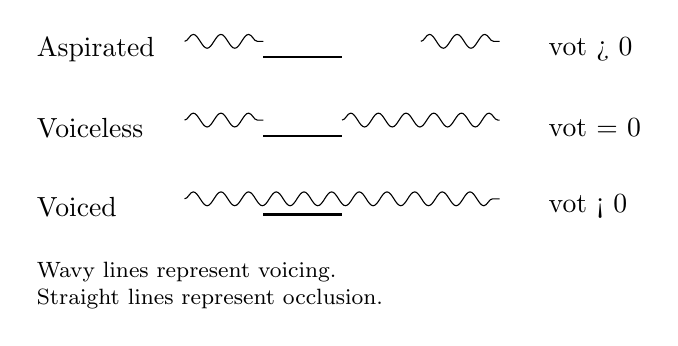
\begin{tikzpicture}
    \tikzset{%
      voicing/.style={yshift=1mm,decorate, decoration={snake}},
      occ/.style={yshift=-1mm,thick},
      descr/.style={anchor=west,align=left}
    }
    \node[descr] (Th) at (0,2) {Aspirated};
    \draw[voicing] (2,2) -- (3,2);
    \draw[voicing] (5,2) -- (6,2);
    \draw[occ] (3,2) -- (4,2);
    \node[descr] (dvot) at (6.5,2) {\gls{vot} > 0};
    \node[descr] (T) at (0,1) {Voiceless};
    \draw[voicing] (2,1) -- (3,1);
    \draw[voicing] (4,1) -- (6,1);
    \draw[occ] (3,1) -- (4,1);
    \node[descr] (dvot) at (6.5,1) {\gls{vot} = 0};
    \node[descr] (D) at (0,0) {Voiced};
    \draw[voicing] (2,0) -- (6,0);
    \draw[occ] (3,0) -- (4,0);
    \node[descr] (dvot) at (6.5,0) {\gls{vot} < 0};
    \node[descr,font=\footnotesize] at (0,-1) {%
      Wavy lines represent voicing.\\
      Straight lines represent occlusion.};
  \end{tikzpicture}
  \caption{Illustration of voiced, voiceless, and aspirated stops.}
  \label{fig:vvadiagram}
\end{figure}
Some languages (\eg Thai) contain three distinct series of phonemes on different points of the \gls{vot} continuum: voiced, voiceless, and voiceless aspirated. It is thus not typologically impossible to have the same phonemic ternary contrast of \gls{vot} in Brittonic, but this is unlikely due to the evidence attesting to length as a variable presented earlier. Given the existence of phonemic length, a two-way phonemic contrast of \gls{vot} is sufficient for immediate post-\gls{apoc} Brittonic.



A stop system with two \gls{vot} grades may also employ intermediate absolute \gls{vot} values between an aspirating/non-aspirating system and a voiceless/voiced system. An example of a language with such a system is English, where aspirating consonants are weakly aspirated compared to their Welsh counterparts, and voiced consonants are weakly voiced, and degree of aspiration and voicing depends on the phonological environment. Figure~\ref{fig:votvarlang} illustrates the various possible configurations. 

\begin{figure}[h]
  \centering
  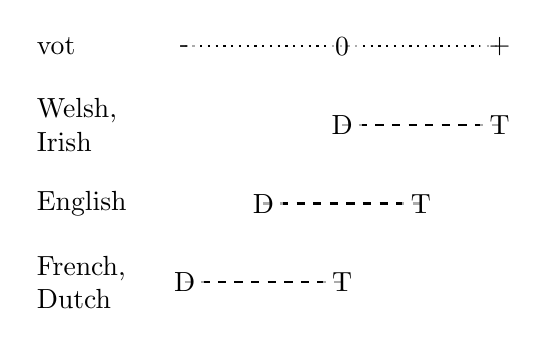
\begin{tikzpicture}
    \tikzset{
      ann/.style={%
        fill=white,
        fill opacity=0.67,
        text opacity=1
      },
      descr/.style={anchor=west,align=left}
    }
    %% LEGEND
    \node[descr] at (0,5) {\gls{vot}};
    \draw[thick, dotted] (2,5) -- (6,5);
    \node[ann] at (2,5) {-};
    \node[ann] at (4,5) {0};
    \node[ann] at (6,5) {+};
    %% LANGS
    \node[descr] at (0,4) {Welsh,\\Irish};
    \draw[thick,dashed] (4,4) node[ann] {\gls{D}} -- (6,4) node[ann] {\gls{T}};
    \node[descr] at (0,3) {English};
    \draw[thick, dashed] (3,3) node[ann] {\gls{D}} -- (5,3) node[ann] {\gls{T}};
    \node[descr] at (0,2) {French,\\Dutch};
    \draw[thick, dashed] (2,2) node[ann] {\gls{D}} -- (4,2) node[ann] {\gls{T}};
  \end{tikzpicture}
  \caption{\Gls{vot} configurations for various languages.}
  \label{fig:votvarlang}
\end{figure}

In \gls{mow}, two phonemic \gls{vot} grades exist: aspirated \mow{p, t, c} and non-aspirated \mow{b, d, g}. All \gls{mob} dialects also have two \gls{vot} grades; the grade with the most delayed \gls{vot} values is represented with \mob{p, t, k}, and the less delayed values with \mob{b, d, g}. Although the absolute \gls{vot} values differ from Breton dialect to dialect, a two-way \gls{vot} opposition of \gls{T} to \gls{D} is maintained in all dialects; the difference between Welsh and Breton dialects with voicing is therefore only quantitative, not structural. Quantitative shifts in \gls{vot} configurations are reasonably common. An example of this is Dutch, a Germanic language which has lost aspiration unlike the majority of Germanic languages. \Textcite[122--123]{Sch_Language14} links this shift to language contact with Romance. Latin and the Romance languages have no aspiration, so Dutch lack of aspiration may simple have been borrowed from Romance. He also notes how unclear the date of Dutch loss of aspiration is; a shift has never been indicated in spelling, because the shift in absolute \gls{vot} values occurred purely at the realisational level and did not entail any structural reorganisation. It is therefore trivial to assume that some Breton dialects similarly shifted towards more advanced \gls{vot} values through language contact with French. This loss of aspiration does not imply any reorganisation either way of consonantal length grades.

The \gls{vot} values of Irish are roughly like those of Welsh~\autocite[85--86]{OD_Irish92}. This means that Irish radical \moi{p, t, c} are strongly aspirating, and \moi{b, d, g} are phonetically weakly voiced or voiceless. As mentioned in Section~\ref{sec:from-brittonic-welsh}, Koch demonstrates that Brittonic \lT\ could be loaned into early Goidelic as \lT\ rather than as \xD. This yielded the stratum of loanwords such as \oi{Cothrige} and \oi{Coirthech}. Later Old Irish did not differentiate between \xT\ and \lT\ by means of voice, but by manner of articulation: \xT\ consisted of stops and \lT\ of fricatives. If Goidelic \xT\ was aspirated, and \lT\ was no more voiced than \xT, it must follow that \lT\ in Goidelic was aspirated in the aforementioned early stratum of loanwords and before it became a fricative. For Brittonic \lT\ to be interpreted as Goidelic \lT, it must have been aspirated. A plain voiceless \lT\ as proposed by Koch would be interpreted as Goidelic \xD. 

\section{My reconstruction}
\label{sec:my-reconstruction}
The identification of voice and aspiration as different realisations of a single variable has consequences for the reconstruction of a post-\gls{apoc} Brittonic stop system. Based on the form of early Brittonic loanwords into Goidelic of the \oi{Coirthech}-type, \textcite{koch_*cothairche_1990} finds that \lT\ cannot have been any more voiced than \xT\ in immediate post-\gls{apoc} Brittonic; that is, \gls{vot} cannot have been lower for \lT\ than \xT, and because we know that \xT\ was aspirated, it must follow that \lT\ was also aspirated. On the basis of this line of reasoning, I propose the stop system in Table~\ref{oldbritishconsonantsystemmine} for immediate post-\gls{apoc} Brittonic.

\begin{table}[h]
  \centering
  \begin{subfigure}[b]{0.5\linewidth}
    \centering
    \begin{tabular}{lll}
      \toprule
      \xT & \xD & \lT \\\midrule
      {[+asp]} & {[-asp]} & {[+asp]}\\
      {[long]} & {[long]} & [short] \\\midrule
      pːʰ & pː & pʰ \\
      tːʰ & tː & tʰ \\
      kːʰ & kː & kʰ \\\bottomrule
    \end{tabular}
    \caption{Concrete notation}
    \label{tab:concrobcmine}
  \end{subfigure}%
  \begin{subfigure}[b]{0.5\linewidth}
    \centering
    \begin{tabular}{lll}
      \toprule
      \xT & \xD & \lT \\\midrule
      {[+\gls{vot}]} & {[-\gls{vot}]} & {[+\gls{vot}]}\\
      {[long]} & {[long]} & [short] \\\midrule
      pː & bː & p \\
      tː & dː & t \\
      kː & ɡː & k \\\bottomrule
    \end{tabular}
    \caption{Abstract notation}
    \label{tab:absobcmine}
  \end{subfigure}
  \caption{The immediate post-\gls{apoc} Brittonic stop system according to myself.}
  \label{oldbritishconsonantsystemmine}
\end{table}


Table~\ref{oldbritishconsonantsystemmine} presents the hypothesised system in two notations. Table~\ref{tab:concrobcmine} contains the more concrete phonetic notation, where the \gls{ipa} symbols are used more literally, so plain \graph{p, t, k} represent any consonant where the \gls{vot} is zero; \graph{ʰ} represents aspirated stops, meaning positive or delayed \gls{vot}. Because  phonetically voiced stops are not found in this system, \graph{b, d, ɡ} are not used. Table~\ref{tab:absobcmine}  represents the same system, but gives a more abstract phonemic notation. Here, \graph{p, t, k} are used where \gls{vot} is comparatively delayed, and \graph{b, d, ɡ} are used where \gls{vot} is comparatively advanced. Thus, the symbols gain meaning in comparison with each other, just like how the values for \gls{vot} gain meaning in comparison with each other in spoken languages. Phonemic transcriptions in this thesis follow the convention laid out in Table~\ref{tab:absobcmine}.

Table~\ref{oldbritishconsonantsystemmine} is hypothesised to be the direct ancestor to derive the \gls{mow} stop system, where only \gls{vot} is phonemic, and where \xT\ is distinct from both \lT\ and \xD\ in \gls{vot}. In order to reach the \gls{mow} stop system from this configuration, two sound laws are needed. The first of these is a redundant rule whereby short consonants are voiced. According to this rule, both initial \lT\ and non-initial \gls{D} became more voiced than \xT. \Textcite{carlyle_syllabic_1988}, who is discussed in Section~\ref{sec:falchun}, posits that such a rule operates synchronically in the phonological computation of Lanhouarneau Breton. In Figure~\ref{fig:pctolbbbstops} in Section~\ref{sec:falchun}, I note how one may reimagine this rule as a diachronic rule in order to derive the Léon Breton word-initial stop system from the \gls{pic} radical and lenited stop allophones proposed by \textcite{harvey_aspects_1984}. Because \xT\ and \lT\ differ in \gls{vot} in \gls{mow} as well as in \gls{mob}, this rule must be extended from  the phonological history of Léon Breton to that of Welsh. As long as this voicing rule was redundant with length, its presence had little effect on the phonology of lenition, because \lT\ was still uniquely marked by its shortness; this is illustrated in Figure~\ref{fig:redvoicvis}. However, its effect became more pronounced when phonemic length was lost, which brings us to the next required sound law.

\begin{figure}[h]
  \centering
  \begin{tikzpicture}
    \draw[->, thick] (0,0) to node[below]{length} (4,0);
    \draw[->, thick] (0,0) to node[left]{\gls{vot}} (0,4);
    \node at (3,1) {\xD};
    \node at (3,3) {\xT};
    \node (ltl) at (1,1) {\lT};
    \node (lte) at (1,3) {\lT};
    \draw[->] (lte) to (ltl);
  \end{tikzpicture}
  \caption{The effects of redundant voicing  visualised}
  \label{fig:redvoicvis}
\end{figure}

The second required sound law is one where length distinctions were lost in the Welsh stop system; this step never occurred in Léon Breton. The second sound law needed is the loss of phonemic length.  This is the sound law that caused the merger between \xD\ and \lT. Redundant voicing of short consonants was fossilised when phonemic length was lost, so loss of phonemic length must postdate redundant voicing, because otherwise the short voiceless stops of \lT\ would merge back with \xT, rather than merging with \xD. Its date is discussed in Part~\ref{part:orthography}.


\section{Overview}
\label{sec:overview-1}

In this introduction I argue how a critical review of earlier scholarship on lenition allows one to posit an original three-way stop opposition between \xT, \xD, and \lT\ in post-\gls{apoc} Brittonic where aspiration and length served to distinguish these series. The middle chapters of Part~\ref{part:phonology-phonetics} serve to confirm the existence of this system in \gls{ow} and early \gls{mw}. These confirmations may also provide a more precise chronology of sound changes than what may be inferred from the secondary literature discussed in this chapter.

Chapter~\ref{oldwelsh} considers the orthography of stops in \gls{ow}. In \gls{ow}, lenition is generally not written, either word-initially or word-internally. Thus, \lT\ is regularly written with \ow{p, t, c}, just like \xT; \lD\ and \xD\ are regularly written with \ow{b, d, g}. This orthography is generally consistent, but there is a handful of instances where \gls{D} is written \ow{p, t, c} and \gls{T} is written with \ow{b, d, g}. The former category comprises all \gls{ow} words containing an etymologically word-internal \xD. Their orthography with \ow{p, t, c} demonstrates that the rare class of word-internal voiced geminates indeed merged with \lT\ as early as the \gls{ow} period. The latter category comprises the minority of words containing word-internal \lT\ spelled with \ow{b, d, g}. Chapter~\ref{oldwelsh} argues that these spellings imply that word-initial \lT\ was distinguished from initial \xD\ by means of aspiration: \lT\ was aspirated and \xD\ was not.

Chapter~\ref{cha:prov-mwbe-y} analyses sandhi patterns of stops in the Poetry of the Princes, which was written from roughly the eleventh century until the thirteenth century. The sandhi patterns found in this corpus  may be studied through the cynghanedd, the system of alliteration in poetry which is still in use today. The present-day cynghanedd  contains some provection rules. Within these rules, the pronunciation of a consonant may change depending on the preceding consonant, and may as a result alliterate with another consonant than itself. Chapter~\ref{cha:prov-mwbe-y} compares how these modern rules differ from the rules of the Poets of the Princes. It finds some differences between the two periods, and proposes a stop phonology within which the earlier rules may be understood. This stop phonology posits both length and aspiration as variables in distinguishing \xT, \lT, and \xD.

% \clearpage
% \begin{itemize}
% \item Finish with Koch:
%   \begin{itemize}
%   \item Account of the evidence Koch finds for \lT≠\xD\ in Welsh
%   \item Account of why Koch argues for /tʰ, t, d/
%   \end{itemize}
% \item Note on Breton use of voice or aspiration to mark T and D

% \item More general discussion of what the difference between a voicing language and an aspirating language are
% \item Perhaps a section on phonological length in MW
  %%% A Section on phonological length in MW???
  % Harvey bases his argument that analogy drove the distinction between \lT\ and \xD\ on the sonorants \mw{r, l, }and \mw{n}. These consonants have two phonemes each: a long fortis, and a short lenis. Naturally then, it is length that distinguishes fortis from lenis here. This identification of length as a marker for fortis quality was then expanded to voiced stops. This matter is of relevance to Welsh, precisely because Welsh does not use length to distinguish fortis and lenis consonants for \mw{r} and \mw{l}. Rather, voice is the common factor in distinguishing \graph{rh} and \graph{r}, and \graph{ll} and \graph{l}, respectively, while \graph{n} does not distinguish between fortis and lenis word-initially\footnote{\gls{mw} does distinguish /nː/, /rː/, and /lː/ from their short counterparts. This distinction is lost before the end of the Middle Welsh period, see also: \textcite[127--128]{schumacher_mittel-_2011}. The relevance of this phonemic opposition for the opposition between lenited voiceless stops and unlenited voiced stops is doubtful, however, because sonorants only use length to distinguish fortis and lenis in non-initial position, whereas it is precisely in word-initial position that lenited voiceless stops and unlenited voiced stops are kept separate in the Early \gls{mw} orthography and in Le Bourg Blanc Breton.}. Resonants  \graph{ll} /ɬ/ and \graph{l} /l/ also differ in manner of articulation: the former sound is a lateral fricative while the latter is a lateral approximant. %% this point is true, but it does not fit here. it talks about the MW situation specifically, so it is more suitable for the conclusion

% \item Conclusion of earlier literature with `state of the art' \ie overview of different viewpoints
% \item Introduction to my own chapters attempting to uncover the phonological variables distinguishing \xT, \lT, \xD.
% \end{itemize}


% \section{Voicing versus aspiration}
% \label{sec:voic-vers-aspir}

% %%% Aspiration in Common Celtic
% Baudiš: Grammar of Early Welsh p.~78
% \Textcite[40, 43, 45]{LP_Concise37}

% %%% On voicing and aspiration in Breton.


% \section{Phonetics and phonology of lenition in present-day Welsh} 
% Unlike Breton, present-day Welsh does not preserve a three-way stop distinction either word-initially or elsewhere. Nevertheless, the way in which the contrast between voiced and voiceless stops is realised phonetically differs between dialects. In some Southeastern dialects of Welsh, the consonants themselves have phonetically merged, but they are kept separate by the length of neighboring vowels: e.g.\ \mw{ebol} /'eːpol/ `foal' v.s. \mw{capel} /'kapel/ `chapel'~\autocite[85]{awbery_phonotactic_1984}. One may wonder whether preceding vowel length similarly played a role in disambiguating the three Early Middle Welsh stop series as it does in disambiguating the two stop series remaining in Modern SE Welsh, and perhaps the modified survival of such a pattern in southeastern Welsh implies that this system survived for longer in these dialects. However, the idea that preceding vowel length may have served to disambiguate lenited voiceless stops from unlenited voiced stops has one drawback: the distinction between three different stop series was only maintained word-initially. The vowel lengthening would therefore have occurred in the word preceding the word to be lenited. The phonetic upshot of this would be (to use Koch's examples~\autocite*[§~26]{koch_*cothairche_1990}): [\c{e}ː g(ː)ar] `her leg' vs. [\c{e} gar] `his car'. This supposition is problematic, because only stressed syllables distinguish between short and long vowels, and the posessive pronouns in the above examples are both unstressed. 


%%% Local Variables:
%%% mode: latex
%%% TeX-master: "../main"
%%% End:
